\section{Entwicklung}

Im Rahmen dieses Software-Projekts sollten wir eine Chrome-Extension entwickeln, die das Ticketsystem der Firma Projektron um KI-Funktionen erweitert. Dazu sollten wir einerseits ein lokales Modell (on-device) und ein externes Modell verwenden.

Wir haben Gemini Nano als lokales und Llama-3.3 als externes Modell verwendet.

\subsection{Gemini Nano}

Gemini Nano ist ein von Google entwickeltes Sprachmodell \cite{gemini-nano}. Der Hauptzweck von Gemini Nano ist es, KI Funktionen clientseitig ausführen zu können, ohne dafür jedesmal ein Sprachmodell herunterladen zu müssen. Dazu wurde Gemini Nano direkt in Chrome Canary integriert. \cite{gemini-nano-build-in-ai}

Aktuell befinden sich Gemini Nano und die dazugehörige API in einer Testphase. In diesem Zustand können und haben sich \footnote{Wie wir mehrfach während der Entwicklung unseres Plugins feststellen mussten} deren Funktionen ständig geändert. \cite{gemini-nano-build-in-ai}

Die Gemini API ist in verschiedene Task API's aufgeteilt. Aktuell sind dies \cite{gemini-nano-apis}:
\begin{itemize}
    \item LanguageDetection
    \item Translation
    \item Summary
    \item Writer + Rewriter
    \item PromptApi \footnote{Unser Plugin stützt sich letzlich auf die PromptApi, auch wenn wir zwischendurch die anderen API's ausprobiert haben.}
\end{itemize} 

\subsection{Dokumentation von Gemini Nano}

Um die oben genannten API's nutzen zu können sollte man dem Origin Trial beiteten. Dies ging über \cite{gemini-nano-origin-trial}. Hier erhiehlten wir die jeweils neuesten Informationen via Email. Dies war notwendig, da die eigentliche Dokumentation \cite{old-doku-language-detection-api, old-doku-translation-api,old-doku-summarization-api,old-doku-writer-api,old-doku-prompt-api} seit längerer Zeit nicht mehr aktuell ist (Stand 04.02.2025). Inzwischen gibt es zwar über \cite{gemini-nano-build-in-ai} eine neue öffentlich zugängliche Dokumentation, allerdings ist diese ebenfalls nicht vollständig.

\subsection{Crome Canary}

Chrome Canary ist die experimentelle Version von Googles Chrome Browser und bietet die Möglichkeit, die neuesten Funktionen zu testen. Canary kann als eine Art Labor betrachtet werden, in dem neue Ideen und Features ausprobiert werden, bevor sie in die endgültige Version von Chrome aufgenommen werden. Diese Vorabversion wird täglich aktualisiert, wodurch die neuesten Entwicklungen stets verfolgt werden können. Da es sich jedoch um eine experimentelle Version handelt, kann es vorkommen, dass Canary instabil ist oder Fehler aufweist \cite{chrome-canary}.

Zum Zeitpunkt der Entwicklung unserer Extension war Chrome Canary die einzige Möglichkeit Gemini Nano zu benutzen.

\subsection{Notwendige Voraussetzungen für Gemini Nano}

Gemini Nano ist unter Windows (10, 11) und unter MacOs (>=13) verfügbar, sofern man mindestens 22 GB freien Speicher hat, über eine GPU verfügt und >= 6 GB VideoRAM hat.

Um Gemini Nano in Chrome Canary nutzen zu können müssen dann mehrere Flags gesetzt werden. Dazu gibt man in der Adresszeile \texttt{chrome://flags} ein. Dort müssen dann folgende Flags gesetzt werden:
\begin{itemize}
    \item Enables optimization guide on device --> \emph{Enabled BypassPerfRequirement}
    \item Text Safety Classifier \footnote{Wenn der Text Safety Classifier nicht ausgeschaltet ist, weigert sich Gemini Nano Texte zu verarbeiten, die nicht in Englsich sind.} --> \emph{Disabled}
    \item Language detection web platform API --> \emph{Enabled}
    \item Experimental translation API --> \emph{Enabled without language pack limit}
    \item Summarization API for Gemini Nano --> \emph{Enabled}
    \item Writer API for Gemini Nano --> \emph{Enabled}
    \item Rewriter API for Gemini Nano --> \emph{Enabled}
    \item Prompt API for Gemini Nano --> \emph{Enabled}
\end{itemize}

Desweiteren sollte man danach in der Adresszeile \texttt{chrome://components/} eingeben und dann \emph{Optimization Guide On Device Model} suchen und aktualisieren.

Um zu testen, ob alles korrekt eingestellt ist und ob man die notwendigen Voraussetzungen erfüllt kann man nun in der Console  des Chrome Browsers \footnote{auf einem Mac: \texttt{Darstellung --> Entwickler --> Java-Script-Konsole}} folgendes eintippen: \texttt{await self.ai.languageModel.availability()} falls man nun \texttt{after-download} oder \texttt{available} als Antwort erhält, kann man Gemini Nano prinzipiell verwenden. Sollte man jedoch \texttt{no} als Antwort bekommen, so wird der verwendete Computer nie in der Lage sein Gemini Nano auszuführen.

\subsection{Chrome Extensions}

Chrome-Extensions \cite{chrome-extensions} sind kleine Softwareprogramme, die die Funktionalität des Google Chrome-Browsers erweitern und an die individuellen Bedürfnisse des Nutzers anpassen. Sie stellen eine Bereicherung des Browser-Erlebnisses dar, indem sie zusätzliche Funktionen implementieren, bestehende modifizieren oder repetitive Aufgaben automatisieren.

Chrome-Extensions basieren auf Webtechnologien wie HTML, CSS und JavaScript. Somit sind sie prinzipiell in jedem Texteditor erstellbar.

\subsection{TypeScript}

Typescript (TS) ist eine von Microsoft entwickelte Erweiterung von JavaScript (JS). \cite{typescript}

TS wird zu JS convertiert, wodurch der geschriebene Code in nahezu jedem Browser läuft. \cite{typescript}

TS erweitert JS durch ein Typsystem in dem unter anderem Interfaces und Klassen beschrieben werden können. Dadurch reduzieren sich die möglichen Fehlerquellen enorm, da der TS-Compiler einfache Typ-Überprüfungen vollziehen kann. Desweiteren ist dadurch auch eine bessere Integration mit IDE's wie zum Beispiel VSCode gegeben. \cite{typescript}

TS ist dabei so entworfen worden, dass jeder gültige JS-Code auch gültiger TS-Code ist. Es ist also möglich ein bestehendes JS-Projekt ohne weiteres auf TS umzustellen. Anschließend kann man, wenn man möchte, den vorhandenen Code zu TS convertieren. \cite{typescript} \cite{ts-doku} Dabei hilft ein Feature von TS. Die so genannte tsconfig.json Datei enthält Einstellungen für den TS-Compiler um beispielsweise erweitertes ErrorChecking zu ermöglichen. \cite{tsconfig}

\subsection{Wie haben wir Typescript genutzt?}

Aufgrund der vielen Vorteile von TS haben wir unsere Chrome Extension direkt und vollständig (100 \%) in TS geschrieben.

Außerdem haben wir die tsconfig.json Datei so eingestellt, dass der TS-Compiler maximal streng vorgeht. Dies bedeutet, dass wir so viele Warnungen und Vorschläge vom Compiler bekommen möchten, wie irgend möglich. Außerdem wurde eingestellt, dass jede Warnung als Fehler zu interpretieren ist und zum Abbruch führt. Für weitere Informationen zur tsconfig.json kann man auf der offiziellen Webseite \cite{tsconfig} nachsehen .

\subsection{Architektur}

\begin{figure}[htbp]
    \centering
    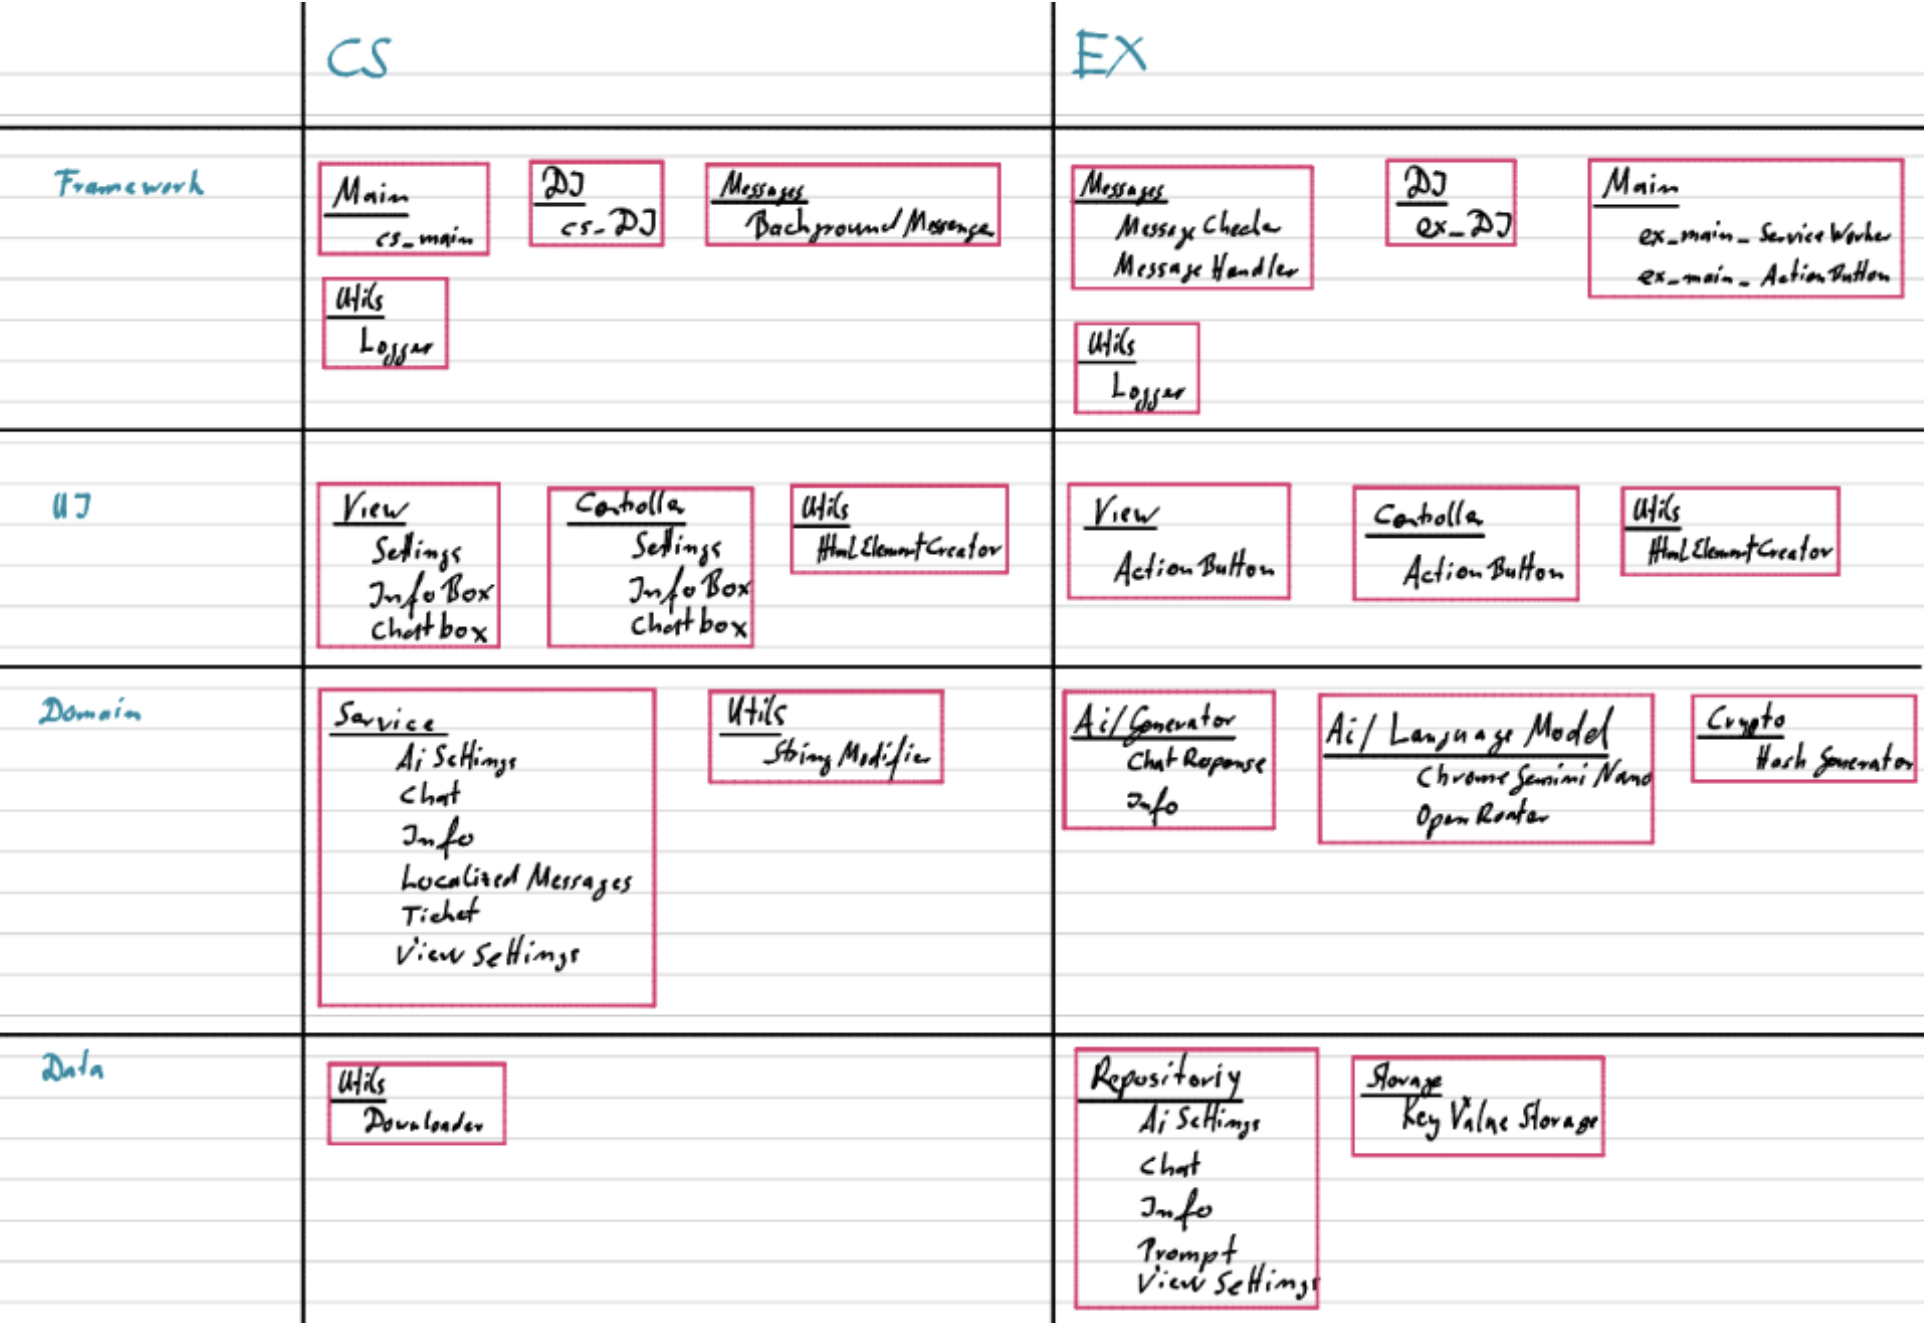
\includegraphics[width=1\textwidth]{img/Architektur.png}
    \caption{Architektur}
    \label{fig:Architektur}
  \end{figure}

  Wir haben unsere Extension nach einem Schichten-Modell aufgebaut, welches eine Daten-, Domain-, UI- und eine Framework-Schicht enthält. Durch die Vorgabe, dass wir eine Chrome-Extension erstellen sollten, gab es zusätzlich noch eine Unterteilung in Content-Script (CS) und Extension-Script (EX) \footnote{Diese Unterteilung haben wir nicht freiwillig getroffen, sondern sie ist eine Notwendigkeit in Chrome-Extensions. }.

  \subsubsection{Content-Script (CS)}

  Das CS in einer Chrome-Extension hat zugriff auf die gerade angezeigte Seite. Dies bedeutet, es ist in der Lage die aktuellen Daten der Seite zu lesen und das DOM der Seite zu manipulieren. Eine der wenigen Chrome-APIs auf die man im CS zugriff hat ist \texttt{hrome.runtime.sendMessage}. Hiermit können Nachrichten an das EX gesendet und auf deren Antwort gewartet werden.

  \subsubsection{Extension-Script (EX)}
  Das EX hat follen Zugriff auf die Chrome-APIs, kann aber nicht auf die aktuelle Seite zugreifen. Es kann Listener registrieren, die auf verschiedene Events reagieren. Zum Beispiel gibt es die Events \texttt{onInstall} und \texttt{onUpdate}, aber auch das Event \texttt{onMessage} \footnote{und weitere Events}. Das letztgenannte Event ermöglicht es die vom CS gesendeten Nachrichten zu verarbeiten. Nach dem erhalt eines Events hat das EX genau 30 Sekunden Rechenzeit \footnote{Dies ist eine harte Randbedingung von Chrome}, bevor es unterbrochen wird.

  \subsubsection{Data-Layer}

  Zu unterst befindet sich bei uns die Data-Layer. Sie ist für das Speichern und Laden der Daten zuständig. Außerdem haben wir hier eigene Datentypen definiert und für jeden zu speichernden Datentyp haben wir ein Repository erstellt. Die Repositories dienen als Abstraktion um zu verbergen, wie und wo die Daten gespeichert werden. Mögliche denkbare Optionen wären lokal vs remote oder Key-Value-Storage vs. Database vs File.

  Während unserer Evaluation der Speicher-Möglichkeiten haben wir uns folgendes überlegt:

  \begin{itemize}
    \item Wir haben nur einen User --> Es ist sehr unwahrscheinlich, dass konkurrierende Zugriffe gemanaged werden müssen.
    \item Selbst wenn Daten überschrieben werden, ist dies egal, da sie von der KI generiert wurden. Und man diesen Vorgang im Zweifel nochmal starten kann.
    \item Mit \texttt{chrome.storage.local} gibt es eine einfach zu nutzende API.
    \item Wir haben keine komplexen Anfragen an den Speicher. Ein Element wird entweder ganz oder gar nicht gebraucht \footnote{Kein \texttt{select, from, where, \dots}}.
  \end{itemize}
  
  Gemäß dem KISS-Prinzip \footnote{Keep It Simple Stupid} haben wir uns daher gegen die Nutzung einer Datenbank und für einen Key-Value-Storage entschieden.

  \subsubsection{Domain-Layer}
  Die zweite Schicht ist die Domain Layer. Hier werden die eigentlichen Aufgaben der Extension ausgeführt.

  Die Domain-Layer bietet bei uns verschieden Service-Klassen an, über die die UI-Layer aufträge erteilen oder Daten erhalten kann. Sie befinden sich im CS. Die Service Klassen selbst verschicken und empfangen hauptsächlich Nachrichten an das EX.

  Im EX wiederum befinden sich zwei Generator-Klassen. Diese dienen als Abstraktion über das verwendete Sprachmodell. Die Aufgabe des Infogenerators besteht darin die statischen Informationen wie Zusammenfassung, Todos oder Termine zu generieren, während der ChatResponse-Generator sich um die antworten des Chatbots kümmert.

  Das zentrale Interface unser Extension ist das LanguageModel. Es stellt folgende Methoden bereit:

  \begin{itemize}
    \item modelName(): Promise<string>
    \item setSystemPrompt(systemPrompt: string): Promise<void>
    \item releaseResources(): Promise<void>;
    \item generate(prompt: string;): Promise<string | undefined>;
    \item maxTokens(): Promise<number>;
    \item countTokens(prompt: string): Promise<number>;
  \end{itemize}

  Die Methode \texttt{setSystemPrompt} bereitet das Sprachmodell auf seine Aufgabe vor. Die Methode \texttt{generate} generiert die eigentliche Antwort des Sprachmodells.

  Die Methoden \texttt{maxTokens} und \texttt{countTokens} sind wichtig um die Länge der Eingabe zu überprüfen, da die meisten Sprachmodelle nur eine begrenzte Menge \footnote{Diese Menge wird in Tokens gemessen. Wir überlassen diese Messung jeweils dem verwendeten Sprachmodell} an Daten verarbeiten können.

  Im Fall von Gemini Nano ist die Methode \texttt{releaseResources} wichtig, da Gemini Nano immer nur von einem Benutzer verwendet werden kann.

  Wir haben in unserer Extension zwei Implementierungen des LanguageModel-Interface. Diese sind ChromeGeminiNano und OpenRouter. OpenRouter ist unsere Wahl um das Remote Modell zu implementieren. Hier werden Http Aufrufe an den Server von Open Router getätigt. Wir übergeben dabei mehere Parameter wie zum Beispiel das gewünschte Sprachmodell und den Prompt und warten dann auf die Antwort des Servers.

  Generell ist unsere Extension so aufgebaut, dass überall nur das Interface LanguageModell verwendet wird. Das heißt außer zum Zeitpunkt der Auswahl des konkreten LanguageModell weiß unsere Extension nie, welches Sprachmodell sie verwendet \footnote{\dots und damit auch nicht, ob die Verarbeitung lokal oder remote erfolgt}. Dies vereinheitlicht und vereinfacht die Verarbeitung der Prompts.

  \subsubsection{UI-Layer}

  In der UI-Layer haben wir die eine strenge Trennung zwischen der Anzeige und der Auswahl der Daten getroffen. Unsere View-Klassen zeigen lediglich Daten an, die an sie übergeben wurden und detektieren Events wie zum Beispiel Clicks. Für die Auswahl der anzuzeigenden Daten, sowie die Reaktion auf die detektierten Events sind unsere ViewController-Klassen zuständig.

  Die ViewController halten außerdem Referenzen auf die Service-Klassen der Domain-Layer. Sie sind  aber lediglich für die Auswahl der Service-Methoden zuständig und geben den Service-Klassen Aufträge.

  \subsubsection{Framework-Layer}

  Als oberste Schicht unser Architektur haben wir eien Framework-Layer eingefügt.